\begin{frame}
	\frametitle{Existence Theory}
	\begin{textblock*}{70mm}(30mm,25mm)
		\begin{greenbox}{}
			$$\left\{ \begin{array}{l}
			\dot{x}(s)=f(s,u(s),x(s))\,\,s\in [t_0,T], \\
			x(t_0)=x_0,\\
			\end{array}
			\right.$$
	
			with terminal state constraint
			$$x(T;t_0,x_0,u(\cdot))\in M, M\subseteq \mathbb{R}^n$$
			
		\end{greenbox}
	\end{textblock*}
	\begin{textblock*}{100mm}(15mm,65mm)
		\begin{yellowbox}{}
			$$J(t_0,x_0;u(\cdot))=\int_{t_0}^{T}g(s,u(s),x(s))ds+h(T,x(T)).$$
		\end{yellowbox}
	\end{textblock*}
\end{frame}
%%%%%%%%%%%%%%%%%%%%%%%%%%%%%%%%%%%%%%%%%%%%%%%%%%%%%%%%%%%%%%%%%%%%%%%%%%%%%%%%

\begin{frame}
	\begin{textblock*}{110mm}(10mm,20mm)
		\begin{graybox}{Problem $(OC)^T$}
			$(t_0,x_0)\in \mathbb{R}_{+}\times \mathbb{R}^n$ with $\tilde{\mathcal{U}}_{x_0}[t_0,T]\neq\emptyset$, find a $\bar{u}(\cdot)\in \tilde{\mathcal{U}}_{x_0}[t_0,T]$ s.t.
			
			\begin{equation*}
				J(t_0,x_0;\bar{u}(\cdot))=\inf_{u(\cdot)\in \tilde{\mathcal{U}}_{x_0}[t_0,T]} J(t_0,x_0;u(\cdot)).
			\end{equation*}
		\end{graybox}
	\end{textblock*}
\end{frame}
%%%%%%%%%%%%%%%%%%%%%%%%%%%%%%%%%%%%%%%%%%%%%%%%%%%%%%%%%%%%%%%%%%%%%%%%%%%%%%%%
\begin{frame}[plain]
	\begin{textblock*}{60mm}(5mm,5mm)
		\begin{graybox}{Hypothesis:}
			\begin{enumerate}[(\textbf{{C}}-1)]
				\item<1->
					$
						f:\mathbb{R}_{+}\times U
						\times \mathbb{R}^n\rightarrow 
						\mathbb{R}^n
					$ is measurable, satisfies a lipchitz
					 condition in $x$,
					$
						|f(t,u,0)|\leq L,\,
						 \forall\,(t,u)\in
						 \mathbb{R}_{+}\times U .
					$
				\item<2->
					$
						g:\mathbb{R}_{+}\times U\times 
						\mathbb{R}^n\rightarrow \mathbb{R},
					$ 
					$
						h:\mathbb{R}^n\rightarrow \mathbb{R}
					$ are measurable, and
					\begin{align*}
						&|g(s,u,x_1)-g(s,u,x_2)|+\\
						&|h(x_1)-h(x_2)|\\
						&\leq \omega(|x_1|\vee |x_2|,|x_1-x_2|)
					\end{align*}
					$
						\forall\, (s,u)\in \mathbb{R}_{+}
						\times U,x_1,x_2\in \mathbb{R}^n
					$.
				\item<3->
					For a.a. $t\in[0,T]$, Cesari property holds $\forall$ $x\in \mathbb{R}^n$.
			\end{enumerate}	
		\end{graybox}
	\end{textblock*}
	\only<2>
	{
		\begin{textblock*}{50mm}(75mm,5mm)
			\begin{yellowbox}{}
				$\omega:\mathbb{R}_{+}\times\mathbb{R}_{+}\rightarrow \mathbb{R}_{+}$, increasing, $\omega(r,0)=0$ $\forall r\geq 0$.
			\end{yellowbox}
		\end{textblock*}
	}
	\only<3>
	{
		\begin{textblock*}{50mm}(75mm,30mm)
			\begin{yellowbox}{}
				\begin{align*}
					&\mathbb{E}(t,x)=\{(z^0,z)\in \mathbb{R}\times \mathbb{R}_{+}|\\
					&z^0\geq g(t,u,x),\\
					&z=f(t,u,x),\, u\in U\}.
				\end{align*}			
			\end{yellowbox}
		\end{textblock*}
	
		\begin{textblock*}{50mm}(75mm,60mm)
			\begin{yellowbox}{Cesari property}
				\begin{equation*}
				\bigcap_{\delta}\bar{co}\mathbb{E}(t,B_{\delta}(x))=\mathbb{E}(t,x)
				\end{equation*}			
			\end{yellowbox}
		\end{textblock*}
	}
\end{frame}
%%%%%%%%%%%%%%%%%%%%%%%%%%%%%%%%%%%%%%%%%%%%%%%%%%%%%%%%%%%%%%%%%%%%%%%%%%%%%%%%

\begin{frame}
	\begin{textblock*}{120mm}(5mm,15mm)
		\begin{graybox}{Existence Theorem}
			Let (C1)-(C3) hold. Then problem $(OC)^T$ admits at least one optimal pair.
		\end{graybox}
	\end{textblock*}
\end{frame}

%%%%%%%%%%%%%%%%%%%%%%%%%%%%%%%%%%%%%%%%%%%%%%%%%%%%%%%%%%%%%%%%%%%%%%%%%%%%%%%%
\begin{frame}
	\begin{equation*}
		H=g(t,x(t),u(t))+\lambda(t)f(t,x(t),u(t)),
	\end{equation*}
	
	\begin{align*}
	H&=A_1I_v+A_2L_p+A_3I_v\sum_{3}^{i=1}c_iu_i^2
	+\lambda_1(-\beta_p S_p I_v +(r +u_1)L_p + (r + u_2) I_p)\\
	&+\lambda_2(\beta_p S_p I_v -b L_p -(r + u_1)L_p)
	+\lambda_3(b L_p - (r + u_2) I_p)\\
	&+\lambda_4(-\beta_v S_v I_p - (\gamma+u_3) S_v -(1-\theta)\mu)
	+\lambda_5(\beta_v S_v I_p -(\gamma+u_3) I_v -\theta\mu).
	\end{align*}
	
\end{frame}
%%%%%%%%%%%%%%%%%%%%%%%%%%%%%%%%%%%%%%%%%%%%%%%%%%%%%%%%%%%%%%%%%%%%%%%%%%%%%%%%
\begin{frame}
	\begin{textblock*}{120mm}(5mm,15mm)
		\begin{graybox}{Pontryagin’s Maximum Principle}
			If $u^*(t)$ and $x^*(t)$ are optimal for the problem $(OC)^T$, then there exists a piecewise differentiable adjoint variable $\lambda(t)$ s.t.
				\begin{equation*}
					H(t,x^*(t),u(t),\lambda(t))\leq H(t,x^*(t),u^*(t),\lambda(t))
				\end{equation*}
			$\forall$ $u$ at $t$,

				\begin{align*}
					\lambda'(t) &= -\frac{\partial H(t,x^*(t),u^*(t),\lambda(t))}{\partial x},\\
					\lambda(T) &= 0.
				\end{align*}
		\end{graybox}
		
	\end{textblock*}
	
\end{frame}

%%%%%%%%%%%%%%%%%%%%%%%%%%%%%%%%%%%%%%%%%%%%%%%%%%%%%%%%%%%%%%%%%%%%%%%%%%%%%%%%

\begin{frame}
	\begin{textblock*}{80mm}(5mm,20mm)
		\begin{graybox}{}
			\begin{align*}
			\frac{d\lambda_1}{dt} &=\beta_p (\lambda_1-\lambda_2),\\
			\frac{d\lambda_2}{dt} &=-A_2+(r+u_1)(\lambda_2-\lambda_1)+b(\lambda_2-\lambda_3),\\
			\frac{d\lambda_3}{dt} &-A_1+(r+u_2)(\lambda_3-\lambda_1)+\beta_vS_v(\lambda_4-\lambda_5),\\
			\frac{d\lambda_4}{dt} &=\beta_v I_p(\lambda_4-\lambda_5)+(\gamma+u_3)\lambda_4,\\
			\frac{d\lambda_5}{dt} &=-A_3+\beta_p S_p(\lambda_1-\lambda_2)+(\gamma+u_3)\lambda_5,				
			\end{align*}
		\end{graybox}	
	\end{textblock*}

	\begin{textblock*}{60mm}(80mm,70mm)
		\begin{greenbox}{}
			$u_1^*=\min\left(\max\left(0,\frac{L_p(\lambda_2-\lambda_1)}{2c_1}\right),u_{1_max}\right)$
			$u_2^*=\min\left(\max\left(0,\frac{I_p(\lambda_3-\lambda_1)}{2c_2}\right),u_{2_max}\right)$
			$u_3^*=\min\left(\max\left(0,\frac{S_v\lambda_4+I_v\lambda_5)}{2c_1}\right),u_{3_max}\right)$
		\end{greenbox}
		
	\end{textblock*}

\end{frame}

%%%%%%%%%%%%%%%%%%%%%%%%%%%%%%%%%%%%%%%%%%%%%%%%%%%%%%%%%%%%%%%%%%%%%%%%%%%%%%%%

\begin{frame}{The most popular}
	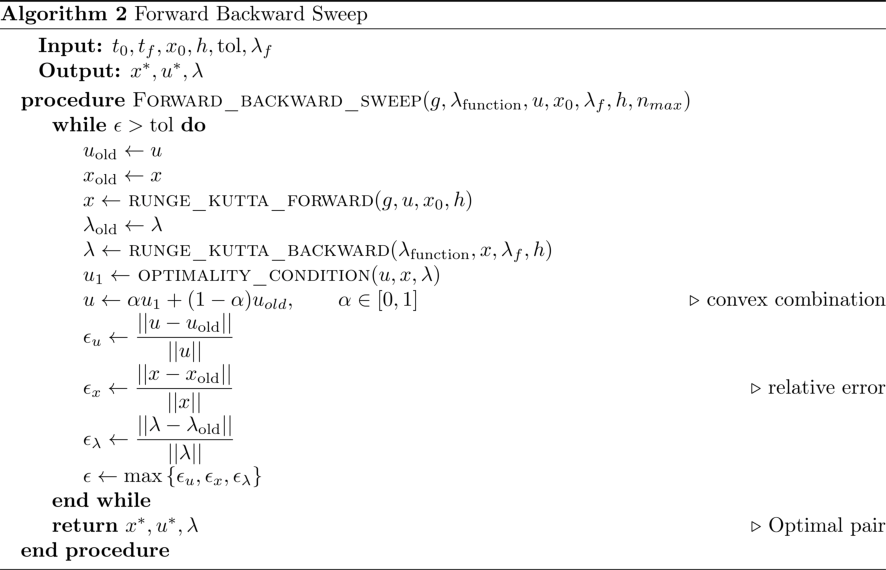
\includegraphics[width=1\linewidth]{Feathergraphics/fbs_algorithm.pdf}
\end{frame}
